\subsection*{Problema 23}

\textbf{Enunciado:} \\
Calcular la integral indefinida:
\begin{align*}
\int \dfrac{\sin^3 x \, dx}{3 - \cos x}
\end{align*}

\textbf{Solución:} \\
Siguiendo las indicaciones, expresamos el término $\sin^3 x$ utilizando la identidad trigonométrica fundamental:
\begin{align*}
\sin^3 x &= \sin^2 x \cdot \sin x \\
&= (1 - \cos^2 x)\sin x
\end{align*}

Sustituimos esta expresión en la integral original:
\begin{align*}
I = \int \dfrac{(1 - \cos^2 x)\sin x}{3 - \cos x} \, dx
\end{align*}

Aplicamos el cambio de variable sugerido:
\begin{align*}
u &= \cos x \\
du &= -\sin x \, dx \implies -du = \sin x \, dx
\end{align*}

Sustituyendo $u$ y $du$ en la integral, obtenemos:
\begin{align*}
I &= \int \dfrac{(1 - u^2)(-du)}{3 - u} \\
&= \int \dfrac{u^2 - 1}{3 - u} \, du
\end{align*}

Para facilitar la integración, reordenamos el denominador como $3 - u = -(u - 3)$ y realizamos la división polinómica o un ajuste algebraico en el numerador sumando y restando $9$:
\begin{align*}
u^2 - 1 &= u^2 - 9 + 8 \\
&= (u - 3)(u + 3) + 8
\end{align*}

Dividimos cada término entre $3 - u$:
\begin{align*}
\dfrac{u^2 - 1}{3 - u} &= \dfrac{-(u - 3)(u + 3) - 8}{3 - u} \\
&= -(u + 3) - \dfrac{8}{3 - u} \\
&= -u - 3 + \dfrac{8}{3 - u}
\end{align*}

Integramos cada término resultante respecto a $u$:
\begin{align*}
I &= \int \left( -u - 3 + \dfrac{8}{3 - u} \right) du \\
&= -\dfrac{u^2}{2} - 3u - 8\ln|3 - u| + C
\end{align*}

Finalmente, regresamos a la variable original $x$ sustituyendo $u = \cos x$:
\begin{align*}
I = &-\dfrac{\cos^2 x}{2} - 3\cos x \\
&- 8\ln|3 - \cos x| + C
\end{align*}

\begin{figure}[H]
	\centering
	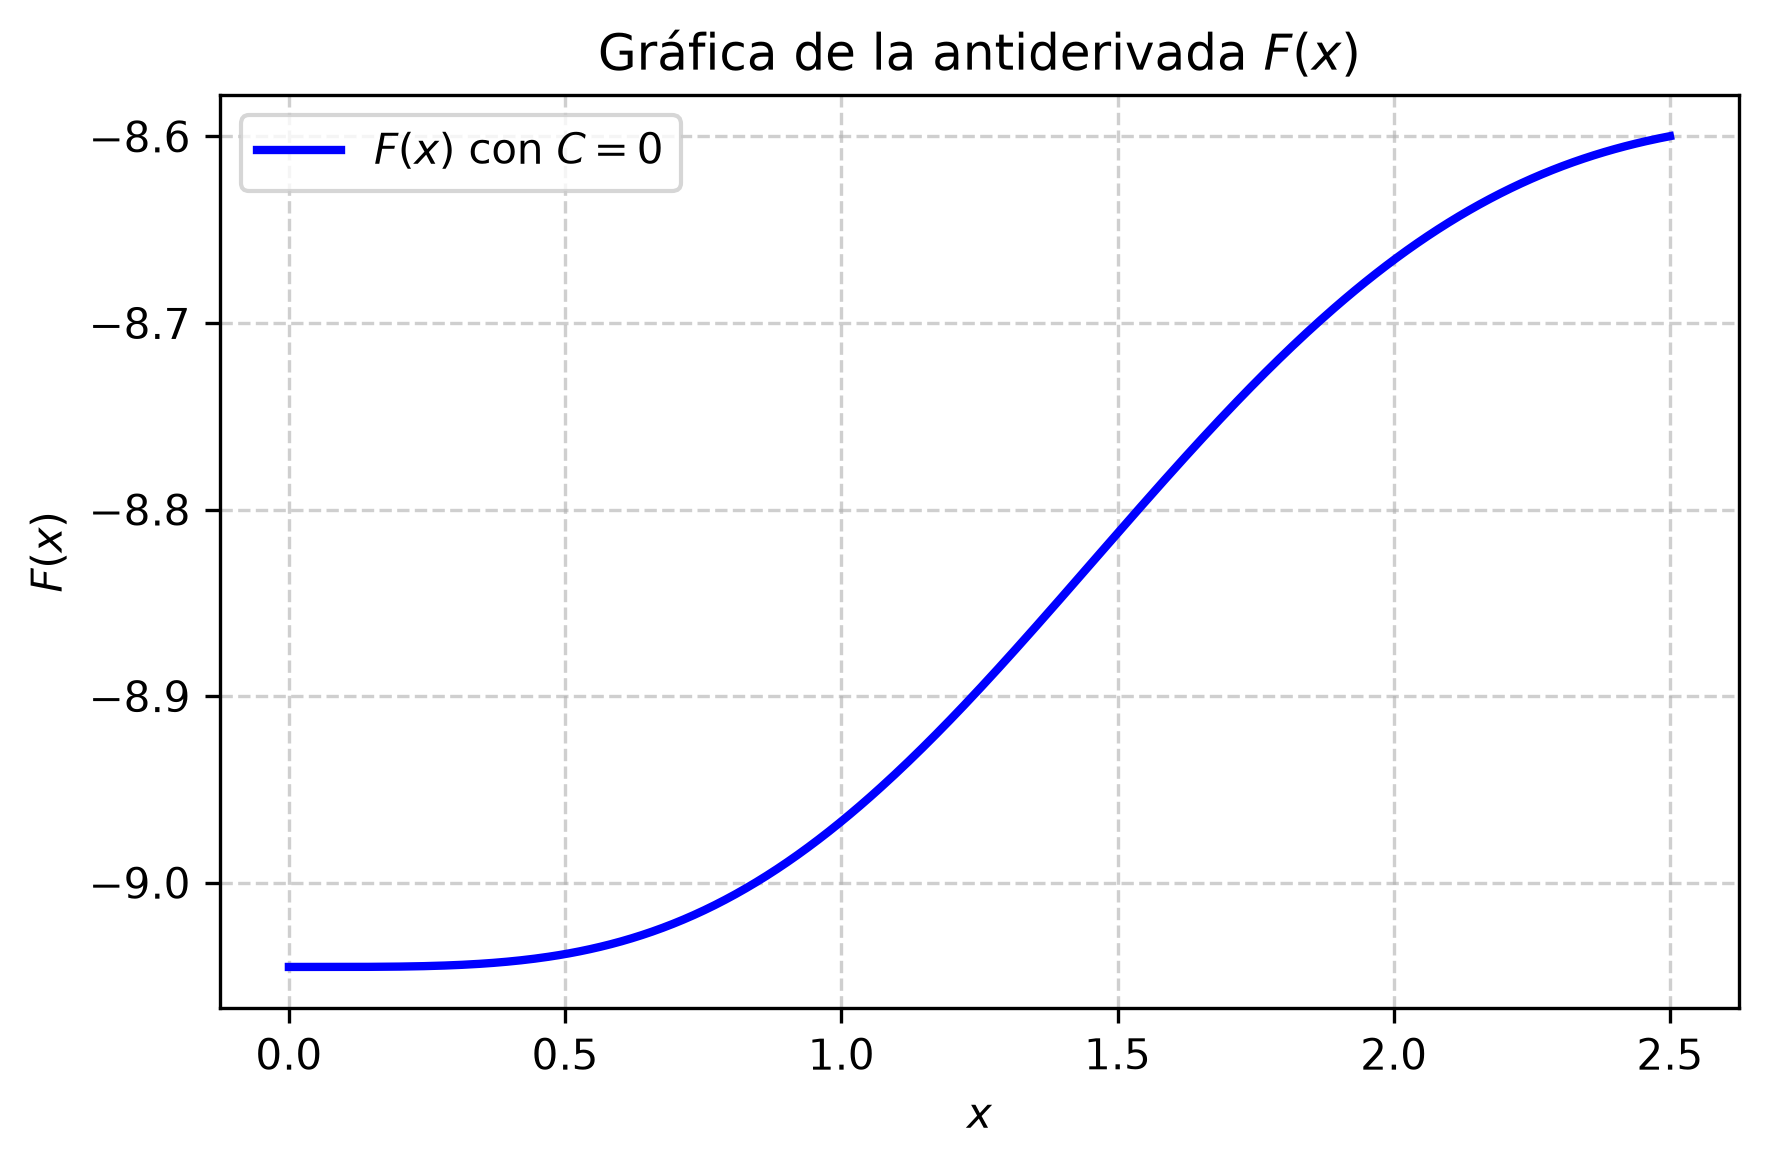
\includegraphics[width=\columnwidth]{semana_04/graficas/SEM04_P23_grafica.png}
	\caption{Representación gráfica de $f(x)$ y su antiderivada $F(x)$ evaluada para la constante de integración $C = 0$ (Problema 23).}
	\label{fig:problema23}
\end{figure}
